% 
% Annual Cognitive Science Conference
% Sample LaTeX Paper -- Proceedings Format
% 

% Original : Ashwin Ram (ashwin@cc.gatech.edu)       04/01/1994
% Modified : Johanna Moore (jmoore@cs.pitt.edu)      03/17/1995
% Modified : David Noelle (noelle@ucsd.edu)          03/15/1996
% Modified : Pat Langley (langley@cs.stanford.edu)   01/26/1997
% Latex2e corrections by Ramin Charles Nakisa        01/28/1997 
% Modified : Tina Eliassi-Rad (eliassi@cs.wisc.edu)  01/31/1998
% Modified : Trisha Yannuzzi (trisha@ircs.upenn.edu) 12/28/1999 (in process)
% Modified : Mary Ellen Foster (M.E.Foster@ed.ac.uk) 12/11/2000
% Modified : Ken Forbus                              01/23/2004
% Modified : Eli M. Silk (esilk@pitt.edu)            05/24/2005
% Modified : Niels Taatgen (taatgen@cmu.edu)         10/24/2006
% Modified : David Noelle (dnoelle@ucmerced.edu)     11/19/2014
% Modified : Roger Levy (rplevy@mit.edu)     12/31/2018



%% Change "letterpaper" in the following line to "a4paper" if you must.

\documentclass[10pt,letterpaper]{article}

\usepackage{cogsci}

%\cogscifinalcopy % Uncomment this line for the final submission 


\usepackage{pslatex}
\usepackage{apacite}
\usepackage{graphicx}
\usepackage{colortbl}
\graphicspath{ {./plots/} }
\usepackage{float} % Roger Levy added this and changed figure/table
                   % placement to [H] for conformity to Word template,
                   % though floating tables and figures to top is
                   % still generally recommended!

%\usepackage[none]{hyphenat} % Sometimes it can be useful to turn off
%hyphenation for purposes such as spell checking of the resulting
%PDF.  Uncomment this block to turn off hyphenation.


\setlength\titlebox{4.5cm}
% You can expand the titlebox if you need extra space
% to show all the authors. Please do not make the titlebox
% smaller than 4.5cm (the original size).
%%If you do, we reserve the right to require you to change it back in
%%the camera-ready version, which could interfere with the timely
%%appearance of your paper in the Proceedings.

\usepackage{booktabs}
\usepackage{color}
\definecolor{LightGray}{gray}{0.92}
\definecolor{Purple}{RGB}{147, 0, 163}
\newcommand{\purple}[1]{\textcolor{Purple}{#1}}
\newcommand{\jd}[1]{\textcolor{Purple}{\bf [jd: #1]}}
\definecolor{Red}{RGB}{163, 0, 0}
\newcommand{\red}[1]{\textcolor{Red}{#1}}
\newcommand{\seb}[1]{\textcolor{Red}{\bf [Seb: #1]}}
\definecolor{Green}{RGB}{0, 176, 76}
\newcommand{\ml}[1]{\textcolor{Green}{\bf [ml: #1]}}

%\renewcommand{\cite}[1]{(\textbf{#1})}

\title{Explaining away in semantic/pragmatic adaptation}
 
\author{{\large \bf Sebastian Schuster ({{sebschu@stanford.edu}}) } \\
   Department of Linguistics, Stanford University\\
   Stanford, CA 94305, USA
  \AND {\large \bf Matthew Iver Loder ({matthew.loder@rutgers.edu})}  \\
  Department of Linguistics, Rutgers University \\
  New Brunswick, NJ 08901, USA
  \AND {\large \bf Judith Degen ({jdegen@stanford.edu})} \\
  Department of Linguistics, Stanford University \\
  Stanford, CA 94305, USA
  }


\begin{document}

\maketitle


\begin{abstract}

Previous work has shown that listeners deal with variability in language use through adaptation; they update expectations about a specific speaker's productions based on the interactions with that speaker. We explore whether contextual information such as a speaker's mood can influence the extent to which listeners adapt to variable use of uncertainty expressions like \textit{might} and \textit{probably}. We find that information about the speaker's mood influences participants' expectations about a generic speaker's use of uncertainty expressions (Exp.~1). We further find that information about the speaker's mood influences adaptation behavior: listeners adapt less to a speaker if they are provided with a reason for the observed language use (Exp.~2), though not more when the behavior is highly unexpected (Exp.~3).  These results suggest that listeners explain away otherwise unexpected behavior when presented with a reason,  and that the extent of adaptation depends on prior expectations about language use.



\textbf{Keywords:} 
adaptation; psycholinguistics; semantics; pragmatics; uncertainty expressions
\end{abstract}


\section{Introduction}

Speakers exhibit production variability at all levels of linguistic representation. Listeners deal with this variability by adapting to speakers and forming speaker-specific expectations about language use \cite<e.g.,>{Norris2003,Kraljic2005,Bradlow2008,Kurumada2012,Kamide2012,Kleinschmidt2015,Fine2016,Roettger2019}. For example, at the lexical level, \citeA{Yildirim2016} found that participants were uncertain whether a generic speaker would use the utterance \textit{Some of the candies are green} or the utterance \textit{Many of the candies are green} to describe a bowl in which there were approximately equal numbers of green and blue candies. However, if participants briefly observed a speaker describing this scene either consistently using \textit{some} or consistently using \textit{many}, they updated their expectations about how that speaker would use quantifiers to describe different proportions. Similarly, \citeA[henceforth S\&D]{Schuster2019} found that listeners update their expectations about a speaker's use of uncertainty expressions like \textit{might} and \textit{probably} after brief exposure to that speaker.

While previous work shows that listeners \emph{can} adapt to variable language use, the contextual conditions and limits on adaptation are under-explored. In principle, it is possible that listeners might update their production expectations regardless of the context of utterance.  Alternatively, listeners' production expectations, and consequently their adaptive behavior, might be modulated by non-linguistic contextual factors. To illustrate this, consider a speaker $S$ who is in a very good mood and wants to be encouraging. If $S$ tells a listener $L$ ``you'll \textit{probably} win the sweepstake'' when there is only a 60\% chance of winning, $L$ may consider $S$'s use of \textit{probably} instead of a weaker alternative such as \textit{might} to be the result of $S$'s mood. Consequently, $L$ would not necessarily expect $S$ to use \textit{probably} to describe the same event probability when $S$ is in a worse or more discouraging mood.

%To illustrate this, consider a listener who encounters a used car salesman describing obviously mediocre cars with highly positive adjectives such as \textit{amazing}. Being aware of the speaker's incentive to use extremely positive language, the listener will likely not update their beliefs about the speaker's use of evaluative adjectives, and for example, if the same speaker later recommends an ``amazing restaurant'', the listener will likely not conclude that the restaurant is actually mediocre.

Recent computational models suggest that adaptation may be modulated by contextual factors. S\&D  proposed a computational model of adaptation to variable use of uncertainty expressions based on Bayesian belief updating. According to this model, when interacting with a speaker and observing their language use, listeners integrate their prior beliefs about the speaker's semantic representations and lexical preferences with the observed utterances to arrive at updated speaker-specific production expectations. Similar Bayesian belief-updating models have been proposed for adaptation in other linguistic domains, including in phonetic adaptation \cite{Kleinschmidt2015}, syntactic adaptation \cite{Kleinschmidt2012}, and prosodic adaptation \cite{Roettger2019}. All of these models predict that the extent to which listeners adapt depends on how they initially expect a speaker to use language. Consequently, contextual factors that affect listeners' expectations about language use should also affect how much listeners adapt to specific speakers. If, given contextual information, a speaker's behavior matches prior expectations, there is no need to adapt.

\begin{figure}
    \centering
    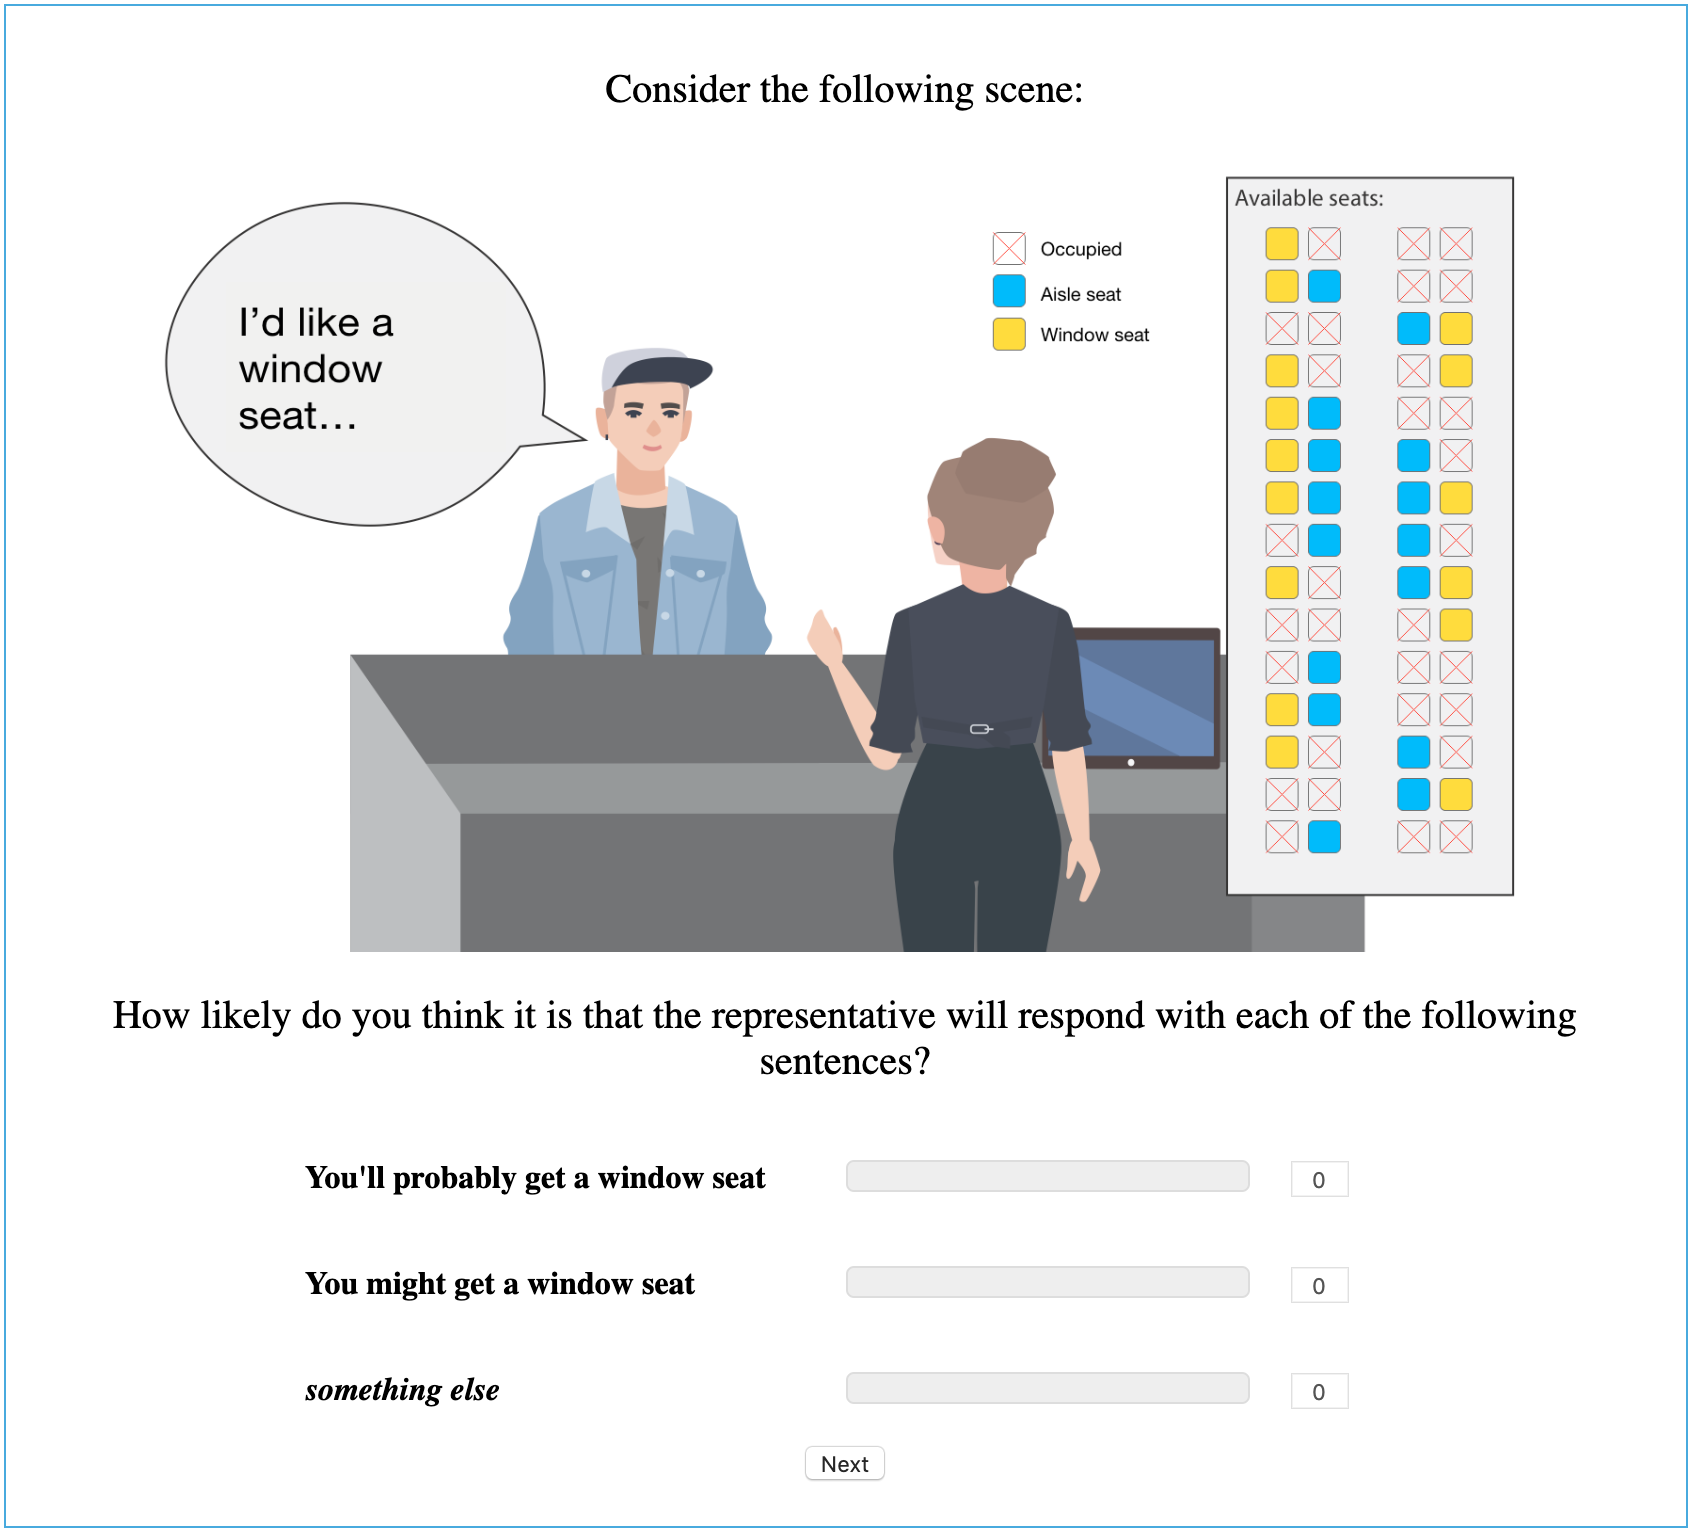
\includegraphics[width=0.9\columnwidth, trim={0 1cm 0 0cm}]{example-trial.png}
    \caption{Example trial from Experiment 1 and the post-exposure blocks from Experiments 2 and 3.}
    \label{fig:example-trial}
\end{figure}

In addition to the model-predicted influence of contextual factors on adaptation, there is  empirical evidence from phonetic adaptation: \citeA{Kraljic2008} used a lexical retuning paradigm to investigate adaptation to a speaker who produced a sound that was ambiguous between /s/ and /sh/. They found that without additional information listeners adapted, such that their perceptual boundary between /s/ and /sh/ shifted. However, when participants were shown a picture of the speaker with a pencil in their mouth, they explained away the observed signal as a pencil-distorted /sh/-sounding /s/ rather than as an intentionally produced /sh/-sounding /s/. Consequently, they did not adapt, i.e., their perceptual boundary between /s/ and /sh/ did not shift.

In this work, we investigate for the first time whether listeners explain away otherwise unexpected behavior at the lexical level if they are presented with contextual information that provides a reason for a speaker's productions. Concretely, we investigate whether one contextual factor  -- the speaker's mood -- provides such a reason for otherwise less expected uses of the uncertainty expressions \textit{might} and \textit{probably}  (\textsc{explaining away hypothesis}). However, considering that previous experimental studies on semantic adaptation \cite{Yildirim2016,Schuster2019} kept all aspects of the context constant between the exposure and test phase, it could also be that listeners simply learn associations between the use of uncertainty expressions and speakers, independent of other contextual information (\textsc{associative hypothesis}).

We investigate this issue as follows. We first establish that language users have different expectations about a generic speaker's use of uncertainty expressions depending on their beliefs about the speaker's mood (Exp.~1). We then investigate how much participants adapt when they are provided with information about the speaker's mood that makes their use of uncertainty expressions more expected, and compare participants' adaptation behavior to a neutral adaptation setting in which participants do not receive any information about the speaker's mood (Exp.~2). Finally, we investigate the relationship between adaptation and highly unexpected behavior by exposing participants to a speaker whose use of uncertainty expressions is incongruent with their mood (Exp.~3). We find that listeners adapt less when they are presented with a reason for the speaker's behavior. However, surprisingly, we also find that listeners do not adapt more when the behavior is highly unexpected given contextual information, potentially suggesting that there are limits on adaptation.

\section{Experiment 1: Effect of speaker mood}

In Exp.~1, we investigated how one contextual factor, the speaker's mood, affects listeners' expectations about a speaker's use of the uncertainty expressions \textit{might} and \textit{probably} for a range of event probabilities. The choice to manipulate the speaker's mood was guided by the intuition that listeners expect a speaker in a good mood to use uncertainty expressions differently from a speaker in a bad mood. Moreover, mood is a non-inherent property of speakers that can change over time, which is important for Exps.~2 and 3. 

Procedure, materials, analyses, exclusions and predictions were pre-registered on OSF (\url{http://osf.io/anonymized}).



\subsection{Methods}

\subsubsection{Participants} We recruited 60 participants (20 per condition) from Amazon's Mechanical Turk. 

%We required participants to have a US-based IP address and an approval rating of at least 95\%, as well as to complete a CAPTCHA at the beginning of the experiment. Participants were paid USD 2.20 (approximately USD 12-15/hr).

\subsubsection{Materials and procedure}
%The paradigm is very similar to \cite{Yildirim2016} and \cite{Schuster2019}\jd{shouldn't this only go into the adaptation experiments?}
At the beginning of the experiment, participants were introduced to an airline representative. Depending on the condition, the instructions explained that the representative was having a particularly bad day and feeling pessimistic and angry (\textit{pessimist} condition); that she was having a particular great day and feeling optimistic and helpful (\textit{optimist} condition); or that she was having a normal day (\textit{neutral} condition). In addition to the textual mood information, the drawing of the representative  showed her with an angry face (\textit{pessimist}), a big smile (\textit{optimist}), or a neutral facial expression (\textit{neutral}).

Participants were then instructed that they would see scenes in which a customer of a cheap airline, who had the choice between getting a seat assigned at random or paying \$50 to pick their seat, would ask the representative about their possible seat assignment, to determine the likelihood of getting their preferred seat without paying. As shown in Fig.~\ref{fig:example-trial}, participants could see the seat map and thus determine the number of available window and aisle seats and estimate the probability of getting the preferred seat. On each trial, participants had to indicate how likely they considered the representative to respond with one of the following two  utterances:

\begin{itemize}
    \item You might get a window seat/an aisle seat. (\textsc{might})
    \item You'll probably get a window seat/an aisle seat. (\textsc{probably})
\end{itemize}

Participants indicated their production expectations by distributing 100 points across these two utterances using a slider. If they thought that neither of the two utterances were likely responses, they could assign points to a blanket \textit{something else} option. Participants completed 36 trials: they provided  4 ratings for each of 9 different probabilities of getting a preferred seat, ranging from 0\% to 100\% as indicated by the seat map. Trials were counterbalanced on whether the customer asked for a window or an aisle seat and trial order was randomized.


\subsubsection{Analysis and exclusions}

Following S\&D, we quantified the production expectations for \textsc{might} and \textsc{probably} by fitting a spline with 4 knots for each participant and expression and computing the area under the curve (AUC) for each of these splines. A larger AUC indicates that an expression was rated highly for a larger range of event probabilities. To compare production expectations across conditions, we computed the difference in AUC between \textsc{might} and \textsc{probably} and compared the average difference across participants in the two conditions.

We excluded participants who provided random responses. Concretely, we excluded participants whose ratings for different event probabilities highly correlated ($r>0.75$) with their average rating, suggesting that they always provided approximately the same rating independent of the event probability. Based on this criterion, we excluded 7 participants (\textit{optimist}: 1, \textit{pessimist}: 3, and \textit{neutral}: 3).

\subsubsection{Predictions}

We predicted that participants expect the \textit{optimistic} speaker to be encouraging and therefore to use \textsc{probably} for a wider range of event probabilities than the \textit{pessimistic} speaker. Conversely, we predicted that participants expect the \textit{pessimistic} speaker to use \textsc{might} for a wider range of probabilities than the \textit{optimistic} speaker. This prediction should be reflected in larger AUC differences in the \textit{pessimist} condition than in the \textit{optimist} condition. Since it was unclear what mood participants attributed to the \textit{neutral} speaker, we only predicted that the mean AUC difference for this third condition should lie between the mean AUC differences of the \textit{optimist} and \textit{pessimist} conditions, with the possibility of being equal to one of the two conditions.

\begin{figure}[t]
    \centering
    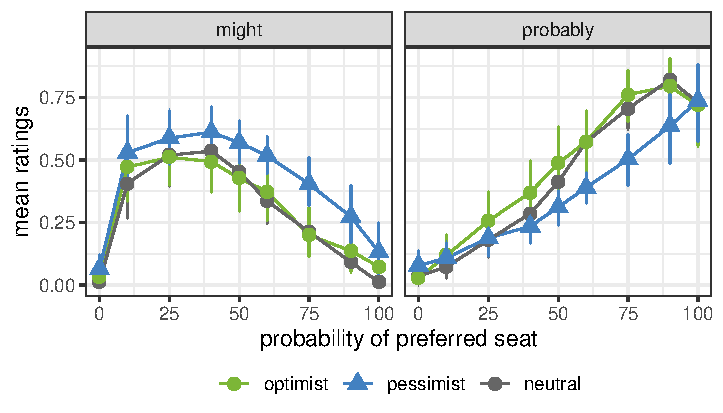
\includegraphics[width=\columnwidth, trim={0 0.75cm 0 0cm}]{norming.pdf}
    \caption{Mean ratings for \textsc{might} and \textsc{probably} for each condition in Exp.~1. Error bars correspond to bootstrapped 95\%-confidence intervals.}
    \label{fig:results-exp1}
\end{figure}

\subsection{Results and discussion}

Fig.~\ref{fig:results-exp1} shows participants' mean ratings for \textsc{might} and \textsc{probably} across the three conditions. As expected, we observe ratings close to 0 for both utterances when there is a 0\% chance of getting the preferred seat (where there is a preference for the \textit{something else} option, not shown), high ratings for \textsc{might} for low event probabilities, and high ratings for \textsc{probably} for high event probabilities. At the same time however, there are also differences across conditions. As the left panel shows, \textsc{might} was rated higher in the \textit{pessimist} condition than in the \textit{optimist} condition for a large range of event probabilities; as the right panel shows, the opposite was true for \textsc{probably}. Ratings in the \textit{neutral} condition were almost identical to the ratings in the \textit{optimist} condition. All these observations were also reflected in the AUC differences: The AUC differences in the \textit{pessimist} condition were greater than in the \textit{optimist} condition ($t(34)=2.51$, $p < 0.05$). The AUC differences in the \textit{neutral} condition -- while numerically slightly larger -- were not significantly different from the differences in the \textit{optimist} condition ($t(34)=0.35$, $p>0.7$).

These results provide evidence that listeners have mood-dependent expectations about a generic speaker's use of uncertainty expressions. In Exp.~2 we investigate whether  speaker mood affects the extent to which listeners adapt to that speaker's use of uncertainty expressions.  %Conditions only differed in the cover story that indicated the speaker's mood, and participants provided different ratings depending on whether they thought the speaker was in a good or bad mood.

%\seb{TODO: relate this to politeness literature.}\jd{not sure this is necessary}

%Given that listeners have different expectations about the production of uncertainty expressions, we expect that information about the speaker's mood also influences the extent to which they adapt to a specific speakers' use of uncertainty expressions. We test this hypothesis in Exp.~2.

\section{Experiment 2: Explaining away}

In an exposure-and-test paradigm, we investigated whether adaptation to a specific speaker is modulated by knowledge about the speaker's mood. We follow S\&D and either exposed participants to a speaker who always used \textsc{might} to describe an event probability of 60\% (henceforth a ``\textit{cautious}'' speaker) or a speaker who always used \textsc{probably} to describe an event probability of 60\% (a ``\textit{confident}'' speaker). Based on the results of Exp.~1, the behavior of a \textit{cautious} speaker is more expected of a speaker who is having a bad day, and the behavior of a \textit{confident} speaker is more expected of a speaker who is having a good day. We thus hypothesized that participants' beliefs about the speaker's mood influence how much they adapt: If the speaker's behavior is mood-congruent, we expected participants to experience a weaker expectation violation and adapt less than in the neutral conditions.

Procedure, materials, analyses, exclusions and predictions were pre-registered on OSF (\url{http://osf.io/anonymized}).

\subsection{Methods}

\subsubsection{Participants} We recruited 320 participants (80 per condition) from Amazon's Mechanical Turk. 

\begin{table}
\begin{tabular}{r|c c|c c }
\toprule 
     \textbf{Condition} & \textit{\textbf{pessimist}} & \textit{\textbf{cautious}} & \textit{\textbf{confident}} & \textit{\textbf{optimist}} \\
     \textbf{Mood} & bad & neutral & neutral & good  \\ \midrule
     $p=25\%$ & \multicolumn{2}{c |}{--} & \multicolumn{2}{c }{\textsc{might} x5} \\
     \cellcolor{LightGray} $p=60\%$ & \multicolumn{2}{c |}{\cellcolor{LightGray} \textsc{might} x5} & \multicolumn{2}{c }{\cellcolor{LightGray} \textsc{probably} x5}\\
     $p=90\%$ & \multicolumn{2}{c |}{\textsc{probably} x5} &  \multicolumn{2}{c }{--} \\
     $p=100\%$ & \multicolumn{2}{c |}{\textsc{bare} x3} & \multicolumn{2}{c }{\textsc{bare} x3} \\
     \bottomrule
\end{tabular}
\caption{Overview of exposure utterances in Exp.~2. $p$ indicates the proportion of preferred available seats shown on the seat map while the speaker produced the utterance. Critical trials are highlighted in gray. \label{tbl:exposure-overview-exp2}}
\end{table}


\subsubsection{Materials and procedure}

The first block of the experiment consisted of an exposure phase with 13 trials (5 critical, 8 filler). On each trial, participants first saw a scene in which a customer asked about a specific seat and a seat map which indicated the number of available window and aisle seats (see top part of Fig.~\ref{fig:example-trial}). To make sure participants paid attention to the seat map, they were then asked to rate how likely the customer  was to get the preferred seat. They then listened to a pre-recorded response from the airline representative. Exposure trials were identical across the \textit{pessimist} and \textit{cautious speaker} conditions and identical across the \textit{optimist} and \textit{confident speaker} conditions but differed across these two pairs of conditions (see Table~\ref{tbl:exposure-overview-exp2} for an overview): In the \textit{pessimist} and \textit{cautious speaker} condition, there were 5 critical trials in which the representative described a 60\% probability of getting the preferred seat with ``You might get one'' (\textsc{might}); in the \textit{optimist} and \textit{confident speaker} conditions, the speaker responded with ``You'll probably get one'' (\textsc{probably}). 5 filler trials in the \textit{pessimist}/\textit{cautious speaker} conditions consisted of \textit{probably} responses   when there was a 90\% preferred seat probability, and 5 filler trials in the \textit{optimist}/\textit{confident speaker} conditions combined \textit{might} with a 25\% preferred seat  probability. Finally, 3 additional filler trials in all four conditions consisted of the response ``You'll get one'' (\textsc{bare}) when it was 100\% likely for the customer to get their preferred seat. Filler trials were intended to boost credibility of the speaker.

The exposure block was followed by another instruction, informing participants in all conditions that it was a week later and that the airline representative was having a normal day, followed by another manipulation check asking participants to rate how they thought the representative was feeling. 

The last block of the experiment was identical to the trials in Exp.~1: participants completed 36 trials and rated how likely they thought it was that the speaker produced \textsc{might}, \textsc{probably} or \textit{something else} for 9 different preferred seat probabilities.

\subsubsection{Analysis and exclusions}

We computed the AUC difference between the splines for  \textsc{might} and \textsc{probably} for each participant as in Exp.~1. We again excluded data from participants providing random responses, which led to 52 exclusions (\textit{pessimist}: 9, \textit{cautious}: 14, \textit{optimist}: 18, \textit{confident}: 11).

\begin{figure}[t]
    \centering
    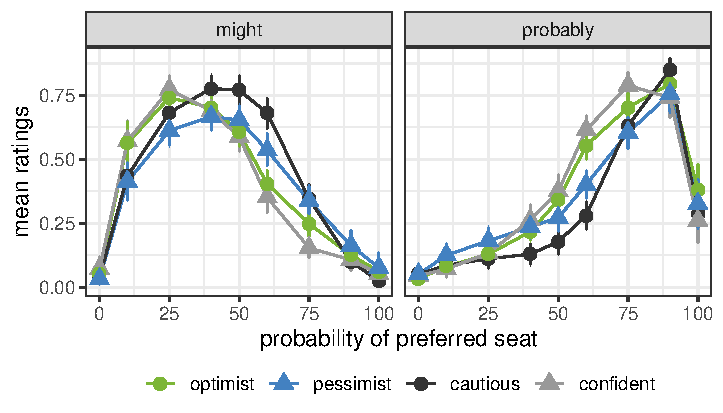
\includegraphics[width=\columnwidth, trim={0 0.75cm 0 0cm}]{explaining-away.pdf}
    \caption{Mean ratings for \textsc{might} and \textsc{probably} for each condition in Exp.~2. Error bars correspond to bootstrapped 95\%-confidence intervals.}
    \label{fig:results-exp2}
\end{figure}
\subsubsection{Predictions}

We expected that participants would adapt to the use of uncertainty expressions by the different speakers and update their expectations. Further, in line with the \textsc{explaining away hypothesis}, participants in the \textit{pessimist} and \textit{optimist} conditions, who should experience less of an expectation violation, should adapt less than participants in the other two conditions. In terms of the AUC difference (AUC(might) - AUC(probably), we therefore expected the following ordering: \textit{cautious speaker} $<$  \textit{pessimist} $\leq$ \textit{optimist} $<$ \textit{confident speaker}.

However, in Exp.~1, we also found that the ratings in the \textit{neutral} condition did not significantly differ from the ratings in the \textit{optimist} condition. This suggests that listeners' initial expectations about the speaker's mood and the associated production expectations only slightly differ across the \textit{optimist} and the \textit{confident speaker} conditions and therefore we also expected similar adaptation behavior in these two conditions.\footnote{This intuition was further confirmed in a pilot study with 10 participants per condition, which we conducted prior to pre-registration. In the pilot, we found the expected ordering for the \textit{cautious speaker}, \textit{pessimist}, and \textit{confident speaker} conditions but the difference between the \textit{optimist} and \textit{confident speaker} condition was so small that we would have needed more than 205 participants per condition to achieve power of $\beta=0.8$.} We therefore, while expecting the numerical ordering described above, expected and pre-registered only significant differences between the \textit{pessimist} and \textit{confident speaker} conditions, and between the \textit{cautious speaker} and \textit{confident speaker} conditions.

If listeners' adaptation behavior is not affected by contextual information, in accordance with the \textsc{associative hypothesis}, there should be no difference between the \textit{cautious speaker} and  \textit{pessimist} conditions and no difference between the \textit{confident speaker} and \textit{optimist} conditions.

\subsection{Results and discussion}

Fig.~\ref{fig:results-exp2} shows the mean ratings for \textsc{might} and \textsc{probably} for the four conditions. The results are consistent with the predictions according to the \textsc{explaining away hypothesis}: First, participants in the \textit{confident speaker} condition rated \textsc{probably} higher for a larger range of event probabilities than in the \textit{cautious speaker} condition and the opposite was true for \textsc{might}. This pattern is also reflected in the mean AUC difference, which is larger in the \textit{cautious speaker} condition than in the \textit{confident speaker} condition ($t(133)=5.18$, $p < 0.001$). This result replicates the adaptation effect found by S\&D and suggests our seat map paradigm is suited for studying adaptation in the use of uncertainty expressions.

Second, we also observe differences between the \textit{cautious speaker} and \textit{pessimist} conditions. The mean AUC difference is larger in the \textit{cautious speaker} condition than in the \textit{pessimist} condition  ($t(135)=2.38$, $p < 0.02$).

Third, we also observe a numeric difference between the \textit{confident speaker} and \textit{optimist} conditions. Numerically, the AUC difference is larger in the \textit{optimist} condition than in the \textit{confident speaker} condition, but not significantly so ($t(129) =1.61$, $p = 0.11$).

Lastly, as shown in Fig.~\ref{fig:manip-check-exp2}, participants in the \textit{optimist} and \textit{pessimist} condition updated their beliefs about the mood after we instructed them that the speaker was now in a normal mood, suggesting that this instruction was sufficient to update participants' beliefs about the speaker's mood. As expected, participants in the two neutral conditions did not change their beliefs about the speaker's mood. 

\begin{figure}[t]
    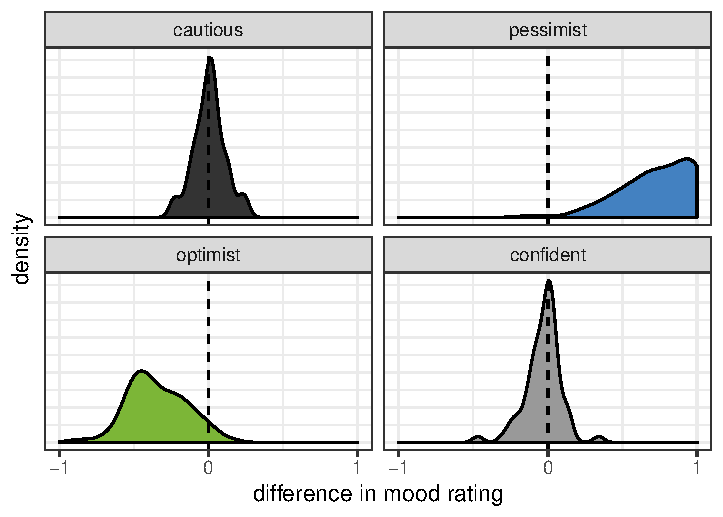
\includegraphics[width=\columnwidth, trim={0 0.75cm 0 0cm}]{mood-differences-exp2.pdf}
    \caption{Differences in mood ratings in Exp.~2. The x-axis indicates the difference between the mood rating before the exposure block and the mood rating before the test block.}
    \label{fig:manip-check-exp2}
\end{figure}


The results from this experiment provide evidence for listeners explaining away otherwise unexpected productions if they are presented with a reason for the speaker's behavior, and are predicted by the \textsc{explaining away} account. 

However, with additional stipulations, these results are also compatible with the \textsc{associative} account. One aspect of the context, the speaker's mood, changed between the exposure block and the test block in the \textit{pessimist} and \textit{optimist} conditions but not in the other two conditions. Therefore, it could be that this difference between the blocks leads to weaker associations between utterances and the context and therefore we observe less adaptation in the \textit{pessimist} and \textit{optimist} conditions. To evaluate this possibility, we conducted Exp.~3.


\section{Experiment 3: Incongruent conditions}

In Exp.~3, we investigated participants' adaptation behavior when the speaker's use of uncertainty expressions was incongruent with the information about the speaker's mood, i.e., a speaker in a bad mood using uncertainty expressions like the \textit{confident speaker} in Exp.~2, or a speaker in a good mood behaving like the \textit{cautious speaker}. According to the \textsc{explaining away} account, this should lead listeners to experience a stronger expectation violation than in the neutral and congruent conditions in the previous experiment and therefore listeners should adapt more.  According to the \textsc{associative} account, on the other hand, listeners should adapt less than in the neutral conditions because according to this account, the smaller adaptation effect that we found in the \textit{optimist} and \textit{pessimist} conditions in the previous experiment was caused by a difference between the exposure phase and the test phase, which is still present in this experiment.


\subsection{Methods}

\subsubsection{Participants} We recruited 160 participants (80 per condition) from Amazon's Mechanical Turk.

\subsubsection{Materials and procedure}

\begin{table}
\centering
\begin{tabular}{r|c | c }
\toprule 
     \textbf{Condition} & \textit{\textbf{pessimist incongr.}} & \textit{\textbf{optimist incongr.}} \\
     \textbf{Mood} & bad  & good  \\ \midrule
     $p=25\%$ & \textsc{might} x5 & -- \\
     \cellcolor{LightGray} $p=60\%$ &  \cellcolor{LightGray} \textsc{probably} x5 & \cellcolor{LightGray} \textsc{might} x5 \\
     $p=90\%$ & -- &  \textsc{probably}  \\
     $p=100\%$ & {\textsc{bare} x3} & {\textsc{bare} x3} \\
     \bottomrule
\end{tabular}
\caption{Overview of exposure utterances in Exp.~3. $p$ indicates the proportion of preferred available seats shown on the seat map while the speaker produced the utterance. Critical trials highlighted in gray.\label{tbl:exposure-overview-exp3}}
\end{table}


The procedure was identical as in Exp.~2. There were two conditions: \textit{optimist incongruent} and \textit{pessimist incongruent}. The \textit{optimist incongruent} condition showed a speaker in a good mood who produced the same utterances as the \textit{pessimist} and \textit{cautious} speaker from the previous experiment. The \textit{pessimist incongruent} condition showed a speaker in a bad mood who produced the same utterances as the \textit{optimist} and \textit{confident} speakers in Exp.~2. See Table~\ref{tbl:exposure-overview-exp3} for an overview of the exposure trials.

\subsubsection{Analysis and exclusions}

Analyses and exclusions were identical to the ones of Exp.~2. We excluded 27 participants (\textit{optimist incongruent}: 15, \textit{pessimist incongruent}: 12).

\subsubsection{Predictions}

We predicted that participants would adapt to different uses of uncertainty expressions: We expected the AUC difference in the \textit{optimist incongruent} condition to be larger than in the \textit{pessimist incongruent} condition. We further predicted that listeners experience a stronger expectation violation than in the neutral conditions in Exp.~2. We therefore also predicted the AUC difference in the \textit{optimist incongruent} condition to be larger than in the \textit{cautious speaker} condition, and the AUC difference in the \textit{pessimist incongruent} condition to be smaller than in the \textit{confident speaker} condition.

\subsection{Results and discussion}

Fig.~\ref{fig:results-exp3} shows the mean ratings for \textsc{might} and \textsc{probably} for the two conditions in this experiment as well as the mean ratings from the neutral conditions from Exp.~2. As this plot shows, participants adapted to the different uses of uncertainty expressions. The mean AUC difference in the \textit{optimist incongruent} condition was larger than in the \textit{pessimist incongruent} condition ($t(131)=5.90$, $p<0.001$). However, unexpectedly, participants did not adapt more in the incongruent conditions than in the neutral conditions. The mean AUC difference in the \textit{optimist incongruent} condition was not larger than in \textit{cautious} condition ($t(129)=0.004$, $p=0.99$), and the mean AUC difference in the \textit{pessimist incongruent} condition was not significantly smaller than in the \textit{confident} condition ($t(135)=-1.18$, $p=0.24$).

\begin{figure}[t]
    \centering
    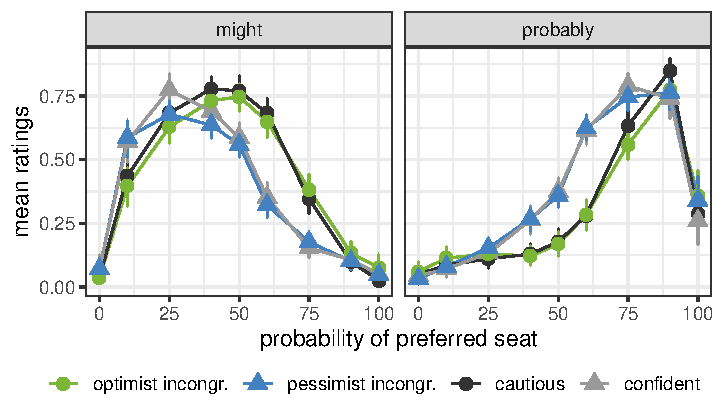
\includegraphics[width=\columnwidth, trim={0 0.75cm 0 0cm}]{incongruent.pdf}
    \caption{Mean ratings for \textsc{might} and \textsc{probably} for the two conditions in Exp.~3 as well as the neutral conditions in Exp.~2. Error bars correspond to bootstrapped 95\%-confidence intervals.}
    \label{fig:results-exp3}
\end{figure}

In this experiment, we again replicated the adaptation effect. However, we did not find a significantly stronger adaptation effect across the two incongruent conditions in this experiment as compared to the neutral conditions from the previous experiment, despite the fact that listeners should have experienced a stronger expectation violation.

What do these results imply for the \textsc{explaining away} and \textsc{associative} accounts that we presented above? Together with the results from Exp.~2, the results from this experiment are unexpected under the \textsc{associative} account: if the reason for participants adapting less in the \textit{pessimist} condition had been the difference in context between the exposure and test blocks, we would have expected less adaptation in this experiment as well.

However, we also did not find stronger adaptation, as we would have expected under the \textsc{explaining away} account. We can only speculate about the reasons for this, but two explanations seem likely. First, given that there was a numerical difference between the \textit{pessimist incongruent} and \textit{confident} conditions in the expected direction, it could be that our experiment was underpowered to detect a potentially very small effect. However, a power analysis suggests we would need more than 500 participants per condition to achieve power of $\beta=0.8$ and therefore we did not explore this option further.

Second, it could be that there is a limit on how much listeners can adapt and that this limit is already reached in the neutral conditions. If this was the case, listeners could still experience a stronger expectation violation when the behavior is incongruent with contextual factors but this stronger violation still does not lead to stronger adaptation. 

%Third, given that the combination of utterances was incongruent with the speaker's mood, and therefore potentially unexpected of a reliable speaker, it could also be that participants were drawing a higher-level inference that the speaker was unreliable \cite<e.g.,>{Grodner2011}.\jd{though this could affect responses in various ways -- is it worth saying this? otherwise perhaps we leave it out after all?}

\section{General Discussion}

In three experiments, we showed that language users have different expectations about the use of uncertainty expressions depending on their beliefs about the speaker's mood, and that this difference in expectations affects the extent of semantic adaptation. The results suggest listeners explain away otherwise unexpected behavior when they are presented with a cause, similarly as \citeA{Kraljic2008} found for phonetic adaptation.

Our results further largely confirm a prediction made by computational models of adaptation, namely that the extent of adaptation depends on how much observed behavior deviates from prior expectations. Similar results have been found for syntactic priming \cite{Jaeger2013} and are predicted by connectionist models of syntactic learning \cite{Chang2006}.

However, the results from Exp.~3 suggest that expectation violation is not the only factor that influences adaptation and that there potentially exist limits to how much listeners can adapt. Investigating the limits of adaptation and developing quantitative linking functions between prior expectations and the extent of adaptation will therefore be important avenues for future work. 

\bibliographystyle{apacite}

\setlength{\bibleftmargin}{.125in}
\setlength{\bibindent}{-\bibleftmargin}

\bibliography{explaining_away}


\end{document}
